\documentclass[class=article, crop=false]{standalone}
% Import packages
\usepackage[margin=1in]{geometry}

\usepackage[many]{tcolorbox}
\usepackage{amssymb, amsthm}
\usepackage{comment}
\usepackage{enumitem}
\usepackage{fancyhdr}
\usepackage{hyperref}
\usepackage{import}
\usepackage{listings}
\usepackage{mathrsfs, mathtools}
\usepackage{pdfpages}
\usepackage{standalone}
\usepackage{transparent}
\usepackage{xcolor}

\usetikzlibrary{decorations.pathreplacing}
\tcbuselibrary{skins}
% Declare math operators
\DeclareMathOperator{\lcm}{lcm}
\DeclareMathOperator{\proj}{proj}
\DeclareMathOperator{\vspan}{span}
\DeclareMathOperator{\im}{im}
\DeclareMathOperator{\range}{range}
\DeclareMathOperator{\Diff}{Diff}
\DeclareMathOperator{\Int}{Int}
\DeclareMathOperator{\fcn}{fcn}
\DeclareMathOperator{\id}{id}
\DeclareMathOperator{\rank}{rank}
\DeclareMathOperator{\tr}{tr}
\DeclareMathOperator{\dive}{div}
\DeclareMathOperator{\row}{row}
\DeclareMathOperator{\col}{col}
% Macros for letters/variables
\renewcommand{\tilde}{\raisebox{0.4ex}{\resizebox{2ex}{!}{\texttildelow}}}
\newcommand{\N}{\ensuremath{\mathbb{N}}}
\newcommand{\Z}{\ensuremath{\mathbb{Z}}}
\newcommand{\Q}{\ensuremath{\mathbb{Q}}}
\newcommand{\R}{\ensuremath{\mathbb{R}}}
\newcommand{\C}{\ensuremath{\mathbb{C}}}
\newcommand{\F}{\ensuremath{\mathbb{F}}}
\newcommand{\M}{\ensuremath{\mathbb{M}}}
\newcommand{\lam}{\ensuremath{\lambda}}
\newcommand{\nab}{\ensuremath{\nabla}}
\newcommand{\eps}{\ensuremath{\varepsilon}}
\newcommand{\es}{\ensuremath{\varnothing}}
% Macros for math symbols
\newcommand{\dx}[1]{\,\mathrm{d}#1}
\newcommand{\inv}{\ensuremath{^{-1}}}
\newcommand{\sm}{\setminus}
\newcommand{\sse}{\subseteq}
\newcommand{\ceq}{\coloneqq}
% Macros for pairs of math symbols
\newcommand{\abs}[1]{\ensuremath{\left\lvert #1 \right\rvert}}
\newcommand{\paren}[1]{\ensuremath{\left( #1 \right)}}
\newcommand{\norm}[1]{\ensuremath{\left\lVert #1\right\rVert}}
\newcommand{\set}[1]{\ensuremath{\left\{#1\right\}}}
\newcommand{\tup}[1]{\ensuremath{\left\langle #1 \right\rangle}}
\newcommand{\floor}[1]{\ensuremath{\left\lfloor #1 \right\rfloor}}
\newcommand{\ceil}[1]{\ensuremath{\left\lceil #1 \right\rceil}}
\newcommand{\eclass}[1]{\ensuremath{\left[ #1 \right]}}

\newcommand{\chapternum}{}
\newcommand{\ex}[1]{\noindent\textbf{Exercise \chapternum.{#1}.}}

\newcommand{\tsub}[1]{\textsubscript{#1}}
\newcommand{\tsup}[1]{\textsuperscript{#1}}

% Include figures
\newcommand{\incfig}[2][1]{%
    \def\svgwidth{#1\columnwidth}
    \import{./figures/}{#2.pdf_tex}
}

\definecolor{problemBackground}{RGB}{212,232,246}

\newenvironment{problem}[1]
  {
    \begin{tcolorbox}[
      boxrule=.5pt,
      titlerule=.5pt,
      sharp corners,
      colback=problemBackground,
      breakable
    ]
    \ifx &#1& \textbf{Problem. }
    \else \textbf{Problem #1.} \fi
  }
  {
    \end{tcolorbox}
  }
\definecolor{exampleBackground}{RGB}{255,249,248}
\definecolor{exampleAccent}{RGB}{158,60,14}
\newenvironment{example}[1]
  {
    \begin{tcolorbox}[
      boxrule=.5pt,
      sharp corners,
      colback=exampleBackground,
      colframe=exampleAccent,
    ]
    \color{exampleAccent}\textbf{Example.} \emph{#1}\color{black}
  }
  {
    \end{tcolorbox}
  }
\definecolor{theoremBackground}{RGB}{234,243,251}
\definecolor{theoremAccent}{RGB}{0,116,183}
\newenvironment{theorem}[1]
  {
    \begin{tcolorbox}[
      boxrule=.5pt,
      titlerule=.5pt,
      sharp corners,
      colback=theoremBackground,
      colframe=theoremAccent,
      breakable
    ]
      \color{theoremAccent}\textbf{Theorem --- }\emph{#1}\\\color{black}
  }
  {
    \end{tcolorbox}
  }
\definecolor{noteBackground}{RGB}{244,249,244}
\definecolor{noteAccent}{RGB}{34,139,34}
\newenvironment{note}[1]
  {
  \begin{tcolorbox}[
    enhanced,
    boxrule=0pt,
    frame hidden,
    sharp corners,
    colback=noteBackground,
    borderline west={3pt}{-1.5pt}{noteAccent},
    breakable
    ]
    \ifx &#1& \color{noteAccent}\textbf{Note. }\color{black}
    \else \color{noteAccent}\textbf{Note (#1). }\color{black} \fi
    }
    {
  \end{tcolorbox}
  }
\definecolor{lemmaBackground}{RGB}{255,247,234}
\definecolor{lemmaAccent}{RGB}{255,153,0}
\newenvironment{lemma}[1]
  {
  \begin{tcolorbox}[
    enhanced,
    boxrule=0pt,
    frame hidden,
    sharp corners,
    colback=lemmaBackground,
    borderline west={3pt}{-1.5pt}{lemmaAccent},
    breakable
    ]
    \ifx &#1& \color{lemmaAccent}\textbf{Lemma. }\color{black}
    \else \color{lemmaAccent}\textbf{Lemma #1. }\color{black} \fi
    }
    {
  \end{tcolorbox}
  }
\definecolor{definitionBackground}{RGB}{246,246,246}
\newenvironment{definition}[1]
  {
    \begin{tcolorbox}[
      enhanced,
      boxrule=0pt,
      frame hidden,
      sharp corners,
      colback=definitionBackground,
      borderline west={3pt}{-1.5pt}{black},
      breakable
    ]
    \textbf{Definition. }\emph{#1}\\
  }
  {
    \end{tcolorbox}
  }

\newenvironment{amatrix}[2]{
    \left[
      \begin{array}{*{#1}{c}|*{#2}c}
  }
  {
      \end{array}
    \right]
  }
\definecolor{codeBackground}{RGB}{253,246,225}
\definecolor{dkgreen}{rgb}{0,0.6,0}
\definecolor{gray}{rgb}{0.5,0.5,0.5}
\definecolor{mauve}{rgb}{0.58,0,0.82}
\lstset{
  language=C++,
  aboveskip=3mm,
  belowskip=3mm,
  backgroundcolor=\color{codeBackground},
  showstringspaces=false,
  columns=flexible,
  basicstyle={\small\ttfamily},
  numbers=none,
  numberstyle=\tiny\color{gray},
  keywordstyle=\color{blue},
  commentstyle=\color{dkgreen},
  stringstyle=\color{mauve},
  breaklines=true,
  breakatwhitespace=true,
  tabsize=2
}

\date{\the\year-\the\month-\the\day}
\author{Kyle Chui}


\fancyhf{}
\lhead{Kyle Chui}
\rhead{Page \thepage}
\pagestyle{fancy}

\begin{document}
  \subsection{Special Functions}
  \begin{definition}{Sequence of elements}
    A sequence in $X$ is a function $s\colon D\to X$ where $D \sse \Z$.
  \end{definition}
  \begin{example}{Sequence}
    \begin{enumerate}[label=(\alph*)]
      \item $X = \set{a, b, c}$, $D = \set{1, 2, 3, 4, 5}$. We may define $s\colon D\to X$ by:
      \begin{align*}
        1 &\mapsto a \\
        2 &\mapsto b \\
        3 &\mapsto c \\
        4 &\mapsto b \\
        5 &\mapsto a
      \end{align*}
      \item The Fibonacci numbers are a sequence of natural numbers. They are defined by: $F_0 = 0, F_1 = 1$, and for $n\geq2$, $F_n = F_{n-1}+F_{n-2}$.
      \item Sequence of even natural numbers: $0, 2, 4, 6, 8, \dotsc$. The function $e\colon \N\to \N$ is defined by $e(n) = 2n$. Observe that the sequence of the powers of 2 is a subsequence of the even natural numbers.
    \end{enumerate}
  \end{example}
  \begin{definition}{Subsequences}
    A \emph{subsequence} of $s\colon D\to X$ is a sequence obtained by restricting the domain of $s$. In other words, a \emph{subsequence} is a sequence of the form $t\colon D'\to X$ where $D' \sse D$.
  \end{definition}
  \begin{definition}{Strings}
    If $X$ is a finite set, a \emph{string} over $X$ is a finite sequence of elements of $X$.
  \end{definition}
  \begin{example}{Strings}
    \begin{enumerate}[label=(\alph*)]
      \item Let $X$ be the English alphabet. Then $c, a, t$ and $d, o, g$ and $m, a, t, h$ are all strings over $X$. We write strings without parentheses and commas, so $c, a, t$ becomes $cat$.
    \end{enumerate}
  \end{example}
  \begin{definition}{Special strings}
    We will let $X^*$ denote the set of strings over $X$. Additionally, let $\lam$ be the null string.
  \end{definition}
  If $\alpha, \beta$ are strings over $X$, we can concatenate them to get a new string $\alpha\beta$.
  \begin{example}{Concatenation}\\
    The string $c, a, t$ concatenated with $d, o, g$ becomes $c, a, t, d, o, g$ or $catdog$.
  \end{example}
  \begin{definition}{Substrings}
    A \emph{substring} is a string obtained by selecting some or all consecutive terms of another string. Observe that the terms must be consecutive, unlike subsequences.
  \end{definition}
  \newpage
  \section{Relations}
  \begin{definition}{Relations}
    A \emph{relation} $R$ from a set $X$ to a set $Y$ is a subset of $X\times Y$. We write $R(x,y)$ or $xRy$ to denote $(x,y)\in R$. If $R$ is a relation from $X$ to $X$, we say that $R$ is a relation on $X$.
  \end{definition}
  \begin{note}{Relations and functions}
    Functions are a special type of relation.
  \end{note}
  \begin{example}{Relations}
    \begin{enumerate}[label=(\alph*)]
      \item Let $X = $ students at UCLA, $Y =$ Classes at UCLA in Winter '21 Quarter. Define $R$ to be a relation between $X$ and $Y$ such that
      \[
      R = \set{(x, y)\in X\times Y\mid x \text{ is a student in }y}.
      \]
      Is $R$ a function? No, because a student can be taking more than one class during the Winter '21 Quarter.
      \item Let $X = \set{2, 3, 4, 5}$ and $Y = \set{4, 5, 6, 7, 8}$. Define the relation $R$ to be: $xRy$ if $x$ divides $y$. Then
      \[
        R = \set{(2, 4), (2, 6), (2, 8), (3, 6), (4, 4), (4, 8), (5, 5)}.
      \]
      \item Let $X = \set{1, 2, 3, 4, 5}$ and define a relation $R$ on $X$ so that $xLy$ if $x < y$. We can visualise this by drawing an arrow $x\rightarrow y$ if $x < y$.
      \begin{center}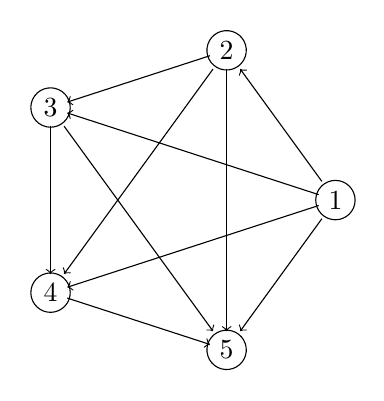
\begin{tikzpicture}
        \draw(2, 0) circle [radius=0.25] node (A) {$1$};
        \draw[rotate=72](2, 0) circle [radius=0.25] node (B) {$2$};
        \draw[rotate=144](2, 0) circle [radius=0.25] node (C) {$3$};
        \draw[rotate=216](2, 0) circle [radius=0.25] node (D) {$4$};
        \draw[rotate=288](2, 0) circle [radius=0.25] node (E) {$5$};
        \draw[->] (A) -- (B);
        \draw[->] (A) -- (C);
        \draw[->] (A) -- (D);
        \draw[->] (A) -- (E);
        \draw[->] (B) -- (C);
        \draw[->] (B) -- (D);
        \draw[->] (B) -- (E);
        \draw[->] (C) -- (D);
        \draw[->] (C) -- (E);
        \draw[->] (D) -- (E);
      \end{tikzpicture}\end{center}
      \item Let $X = \set{1, 2, 3, 4, 5}$, and define a relation $LE$ on $X$ such that $xLEy$ if $x\leq y$. The diagram is the exact same as above, but every element is also related to itself (because $x\leq x$ for all $x$).
    \end{enumerate}
  \end{example}
  \subsection{Types of Relations}
  \begin{enumerate}[label=(\alph*)]
    \item Reflexive: $R$ is reflexive if for all $x\in X$, $xRx$ ($x$ relates to itself).
    \item Symmetric: $R$ is symmetric if for all $x, y\in X$, $xRy\implies yRx$.
    \item Antisymmetric: $R$ is antisymmetric if for all $x, y\in X$, $xRy$ and $yRx$ implies $x = y$.
    \item Transitive: $R$ is transitive if for all $x, y, z\in X$, $xRy$ and $yRz$ implies $xRz$.
  \end{enumerate}
  \begin{example}{Types of relations}
    \begin{enumerate}[label=(\alph*)]
      \item The relation $<$ over the reals is transitive, (vacuously) antisymmetric, not symmetric, and not reflexive.
      \item The relation $\leq$ over the reals is transitive, antisymmetric, not symmetric, and not reflexive.
      \item Let $X =$ people, and $xNy$ if $x$ and $y$ have the same name. Then $N$ is reflexive, symmetric, and transitive.
      \item Let $X =$ people, and $xTy$ if $x$ is taller than $y$. Then $T$ is transitive, because if $x$ is taller than $y$, and $y$ is taller than $z$, then $x$ is taller than $z$.
    \end{enumerate}
  \end{example}
  \begin{definition}{Inverse of a relation}
    If $R$ is a relation from $X$ to $Y$, then $R\inv$ is the relation from $Y$ to $X$ defined by:
    \[
      R\inv = \set{(y, x)\in Y\times X\mid (x, y)\in R}.
    \]
  \end{definition}
  \begin{definition}{Composition of relations}
    If $R\sse X\times Y$, and $S\sse Y\times Z$, then $S\circ R\sse X\times Z$ such that
    \[
      S\circ R = \set{(x, z)\in X\times Z\mid \text{there exists $y\in Y$ such that $(x,y)\in R$ and $(y,z)\in S$}}.
    \]
  \end{definition}
  \begin{definition}{Equivalence relation}
    A relation is an \emph{equivalence relation} if it is reflexive, symmetric, and transitive.
  \end{definition}
\end{document}
